\section{Převodník USB-UART CP2102N}
\label{sec:prevodnik-usb-uart-cp2102n}
Pro programování nástěnného snímače prostorové teploty, přesněji modulu ESP32 Wrover-IE je použit převodní USB-UART CP2102N \cite{cp2102n-miniek} od firmy Silocon Labs. Zakoupil jsem již hotový modul CP2102N MINEK (obrázek \ref{fig:prevodnik-cp2102n-modul-vrchni-cast}). Modul je doplněn o zapojení tranzistoru pro automatický reset a automatický boot modulu (obrázek \ref{fig:prevodnik-cp2102n-modul-spodni-cast}). Z modulu se využívají signály \acrshort{dtr} (\textit{\acrlong{dtr}}) a \acrshort{rts} (\textit{\acrlong{rts}}). Pokud je potřeba vstoupit do bootloaderu pro nahrání nového firmwaru, je nutné podržet boot a~následně stisknout reset, zařízení je tak připraveno nahrát nový firmware. V případě využití signálu DTR a RTS se tato operace dělá automaticky, nicméně z~pravdivostní tabulky \ref{tab:pravdivostni-tabulka-pro-automaticky-boot} není vidět stav pro EN = 0, IO0 = 0, tento stav je zajištěn pomocí kondenzátoru o velikosti 1\textmu  F mezi EN vstup a~GND. Tímto kondenzátorem se zajistí zpoždění při přechodu z log. 0 na log. 1 na vstupu EN, zároveň v~tomto zpoždění je vstup IO0 v log. 0 a je možné vstoupit do bootloaderu. Z modulu jsou do konektoru vyvedeny 5 V, GND, RXD, TXD, EN a IO0. Komunikace mezi CP2102N a modulem ESP32 pak probíhá po vodičích RXD a TXD. Schéma zapojení pro automatický bootloader s~využitím modulu CP2102N MINEK je v příloze \ref{app:schemata-ostatni}.

\begin{center}
\begin{table}[H]
\begin{tabular}{ |c|c||c|c| }  
 \hline
 \thead{DTR} & \thead{RTS} & \thead{EN} & \thead{IO0}\\
 \hline
 1 & 1 & 1 & 1 \\ 
 0 & 0 & 1 & 1 \\ 
 1 & 0 & 0 & 1 \\ 
 0 & 1 & 1 & 0 \\ 
 \hline
\end{tabular}
 \caption{Pravdivostní tabulka pro automatický boot modulu ESP32.}
 \label{tab:pravdivostni-tabulka-pro-automaticky-boot}
\end{table}
\end{center}


%\begin{figure}[H]
%    \centering
%    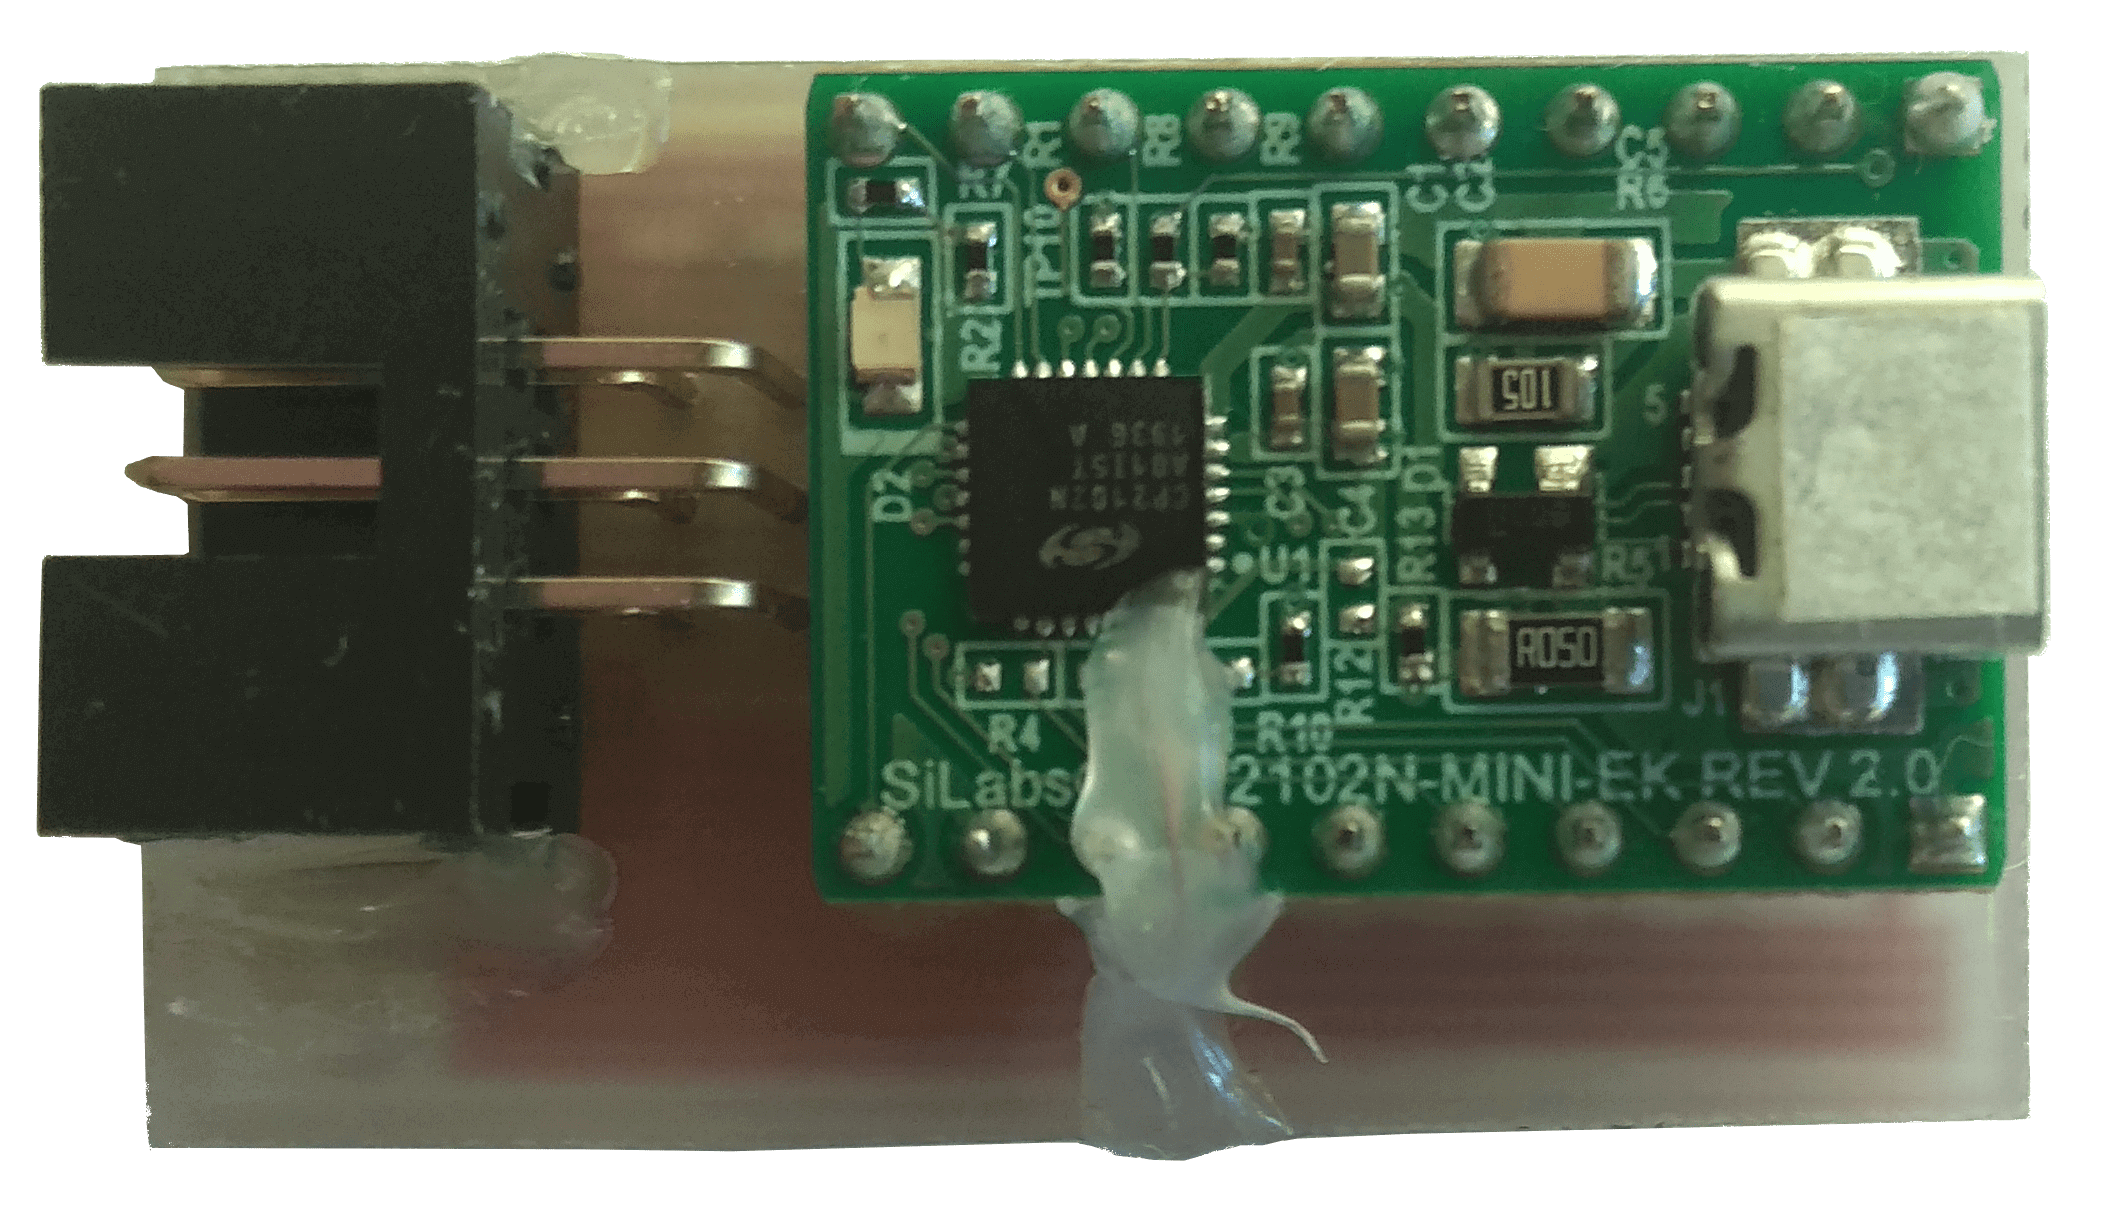
\includegraphics[width=0.5\textwidth]{images/prevodnik-usb-uart-cp2102n/prevodnik-cp2102n-modul-vrchni-cast.png}
%    \caption[Vrchní část modulu převodníku USB-UART.]{Vrchní část modulu převodníku USB-UART CP2102N MINEK s~výstupním konektorem pro programování zařízení.}
%    \label{fig:prevodnik-cp2102n-modul-vrchni-cast}
%\end{figure}


%\begin{figure}[H]
%    \centering
%    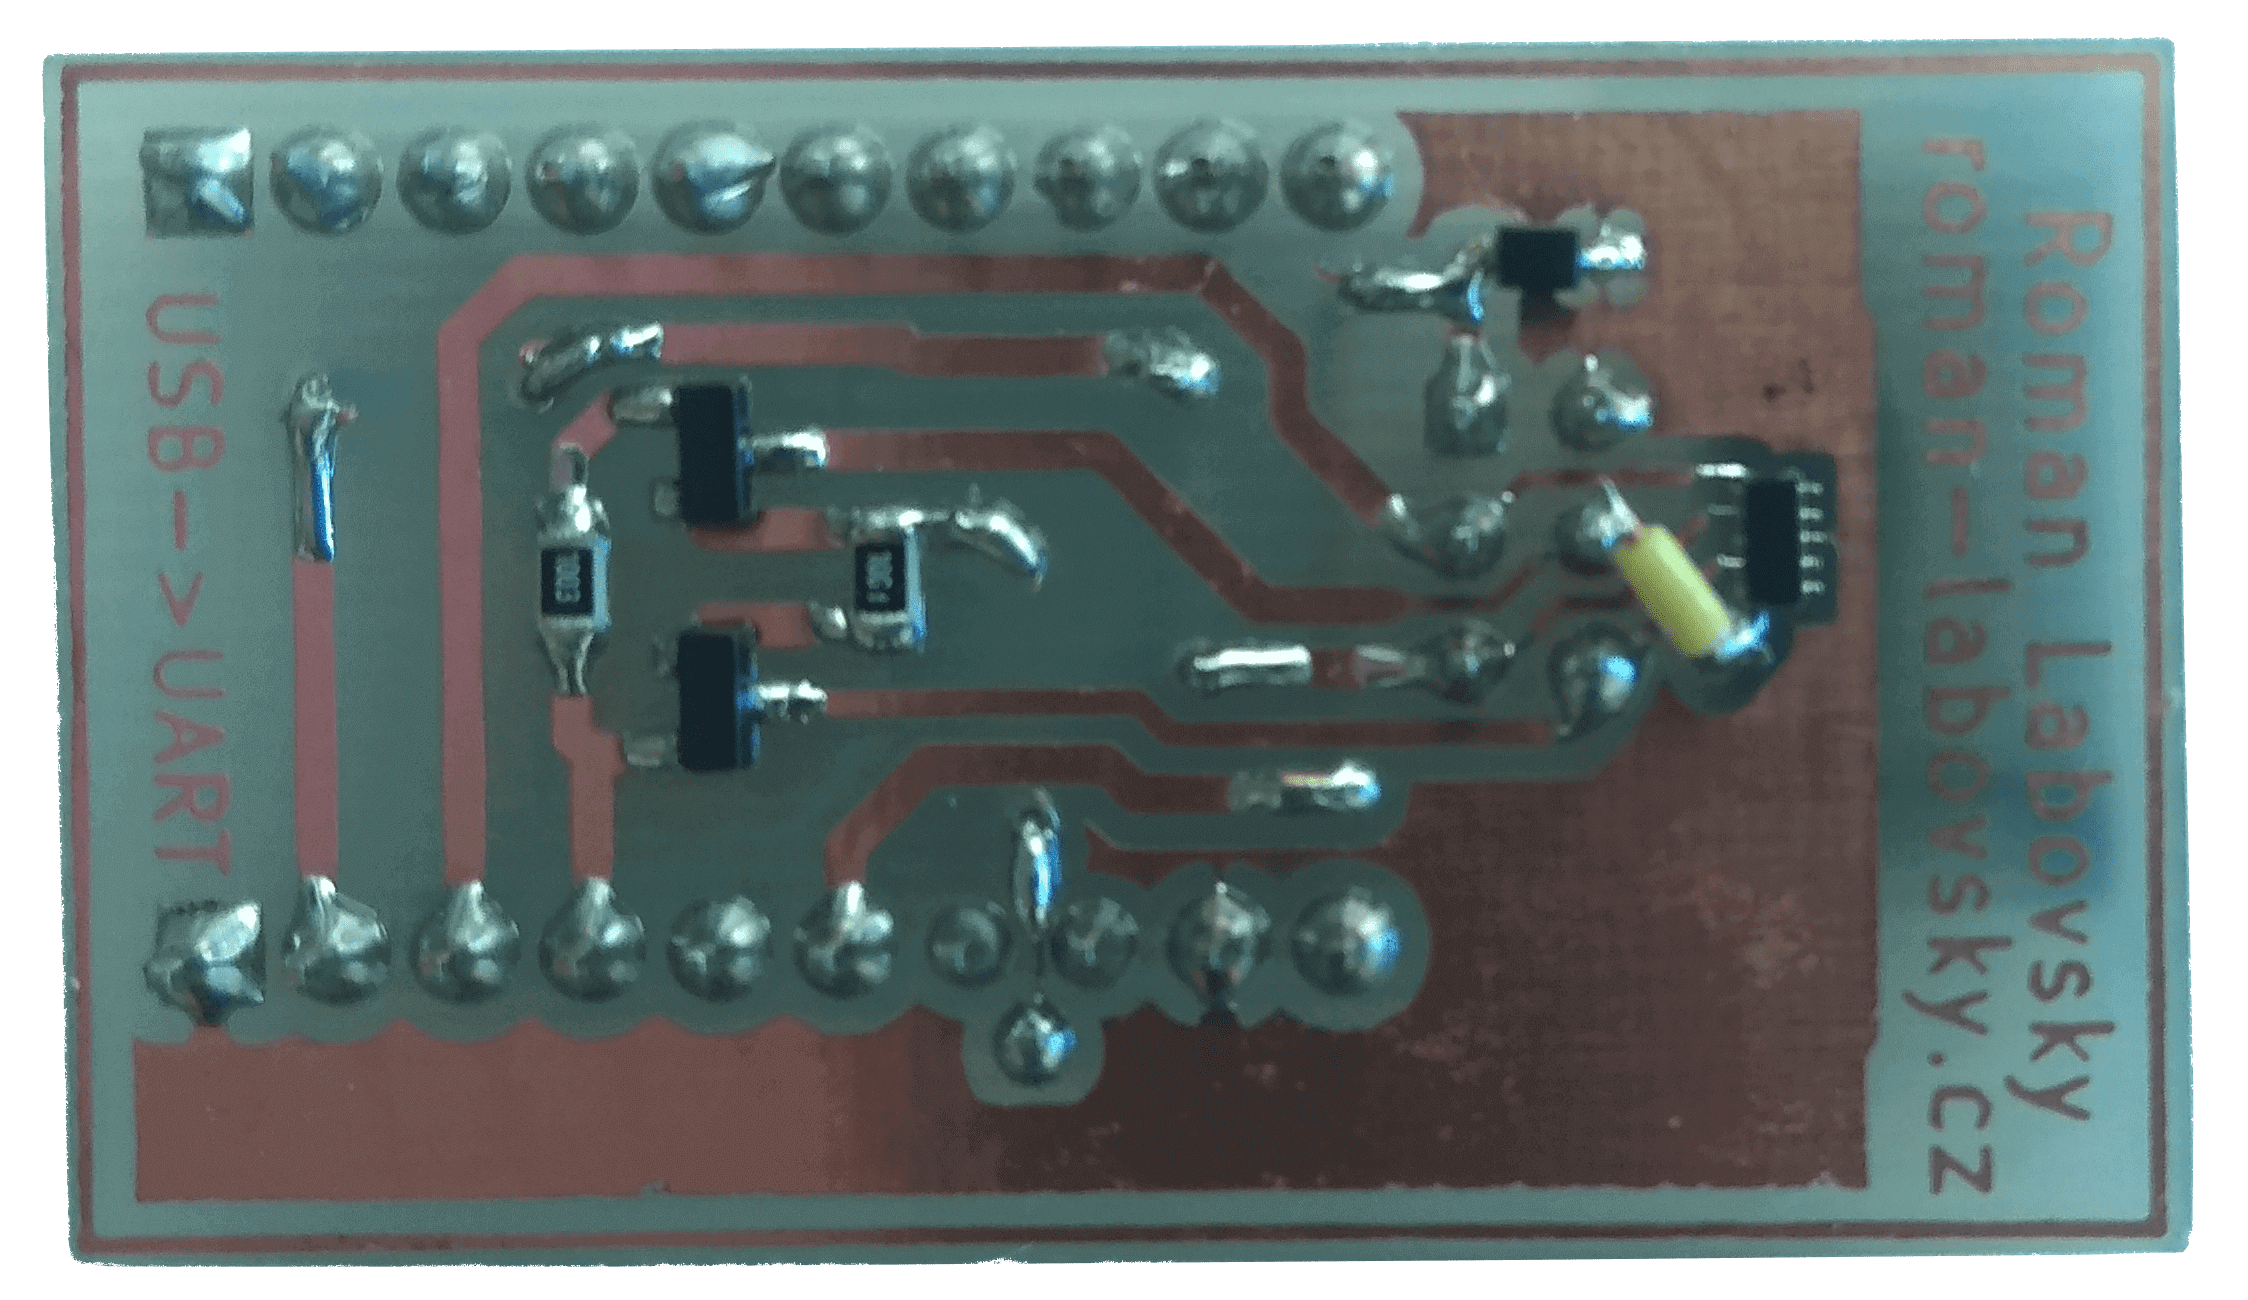
\includegraphics[width=0.5\textwidth]{images/prevodnik-usb-uart-cp2102n/prevodnik-cp2102n-modul-spodni-cast.png}
%    \caption[Spodní část modulu převodníku USB-UART.]{Spodní část modulu převodníku USB-UART s doplněnými tranzistory pro signály DTR a RTS pro automatický bootloader.}
%    \label{fig:prevodnik-cp2102n-modul-spodni-cast}
%\end{figure}



\begin{figure}[H]
\centering
\begin{subfigure}{.5\textwidth}
    \centering
    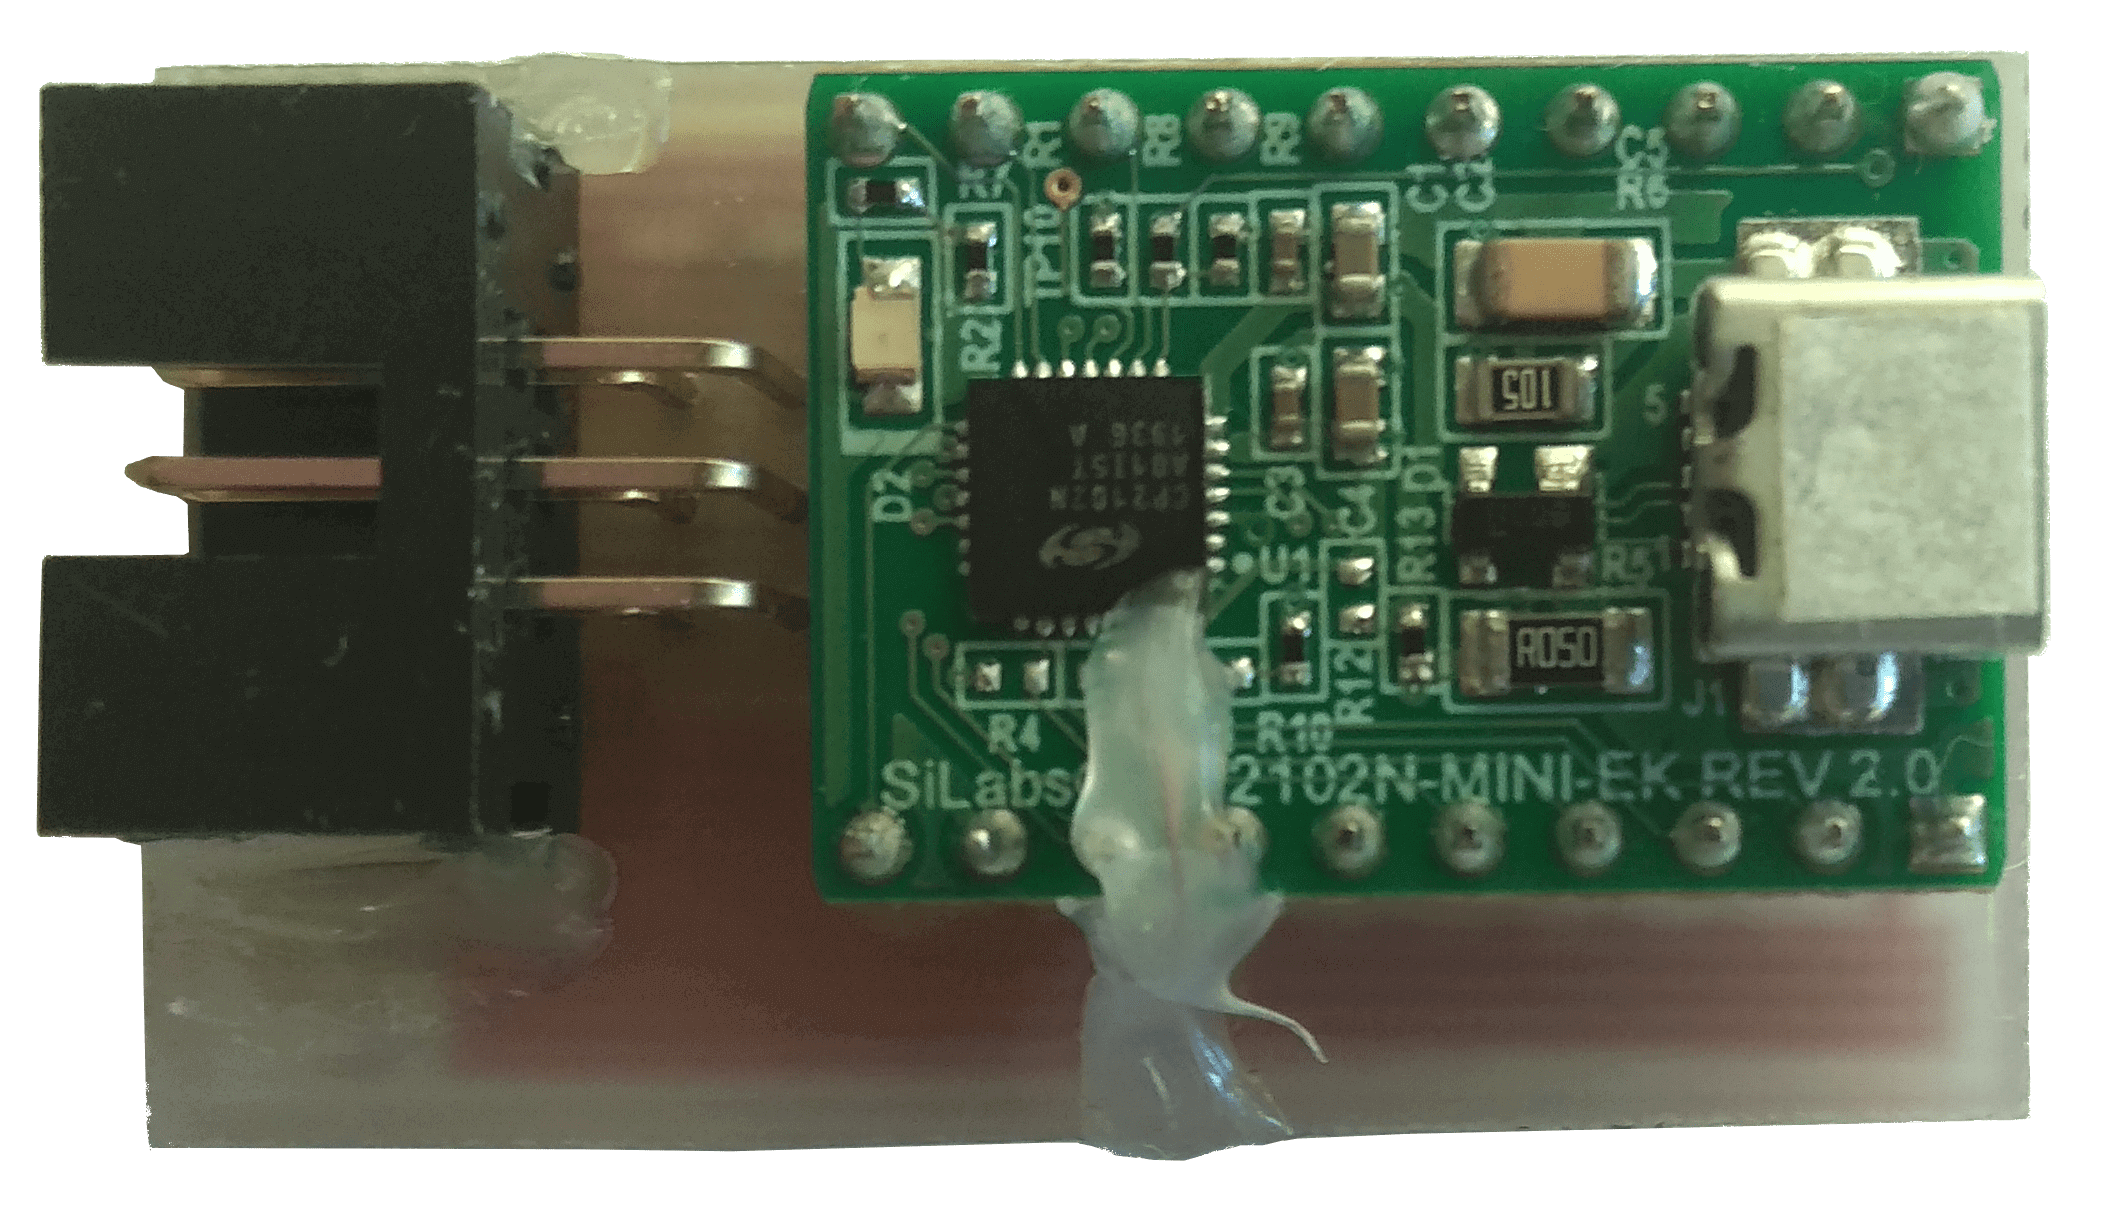
\includegraphics[width=\textwidth]{images/prevodnik-usb-uart-cp2102n/prevodnik-cp2102n-modul-vrchni-cast.png}
    \caption[Vrchní část modulu převodníku USB-UART.]{Vrchní část modulu převodníku USB-UART CP2102N MINEK s~výstupním konektorem pro programování zařízení.}
    \label{fig:prevodnik-cp2102n-modul-vrchni-cast}
\end{subfigure}%
\begin{subfigure}{.5\textwidth}
    \centering
    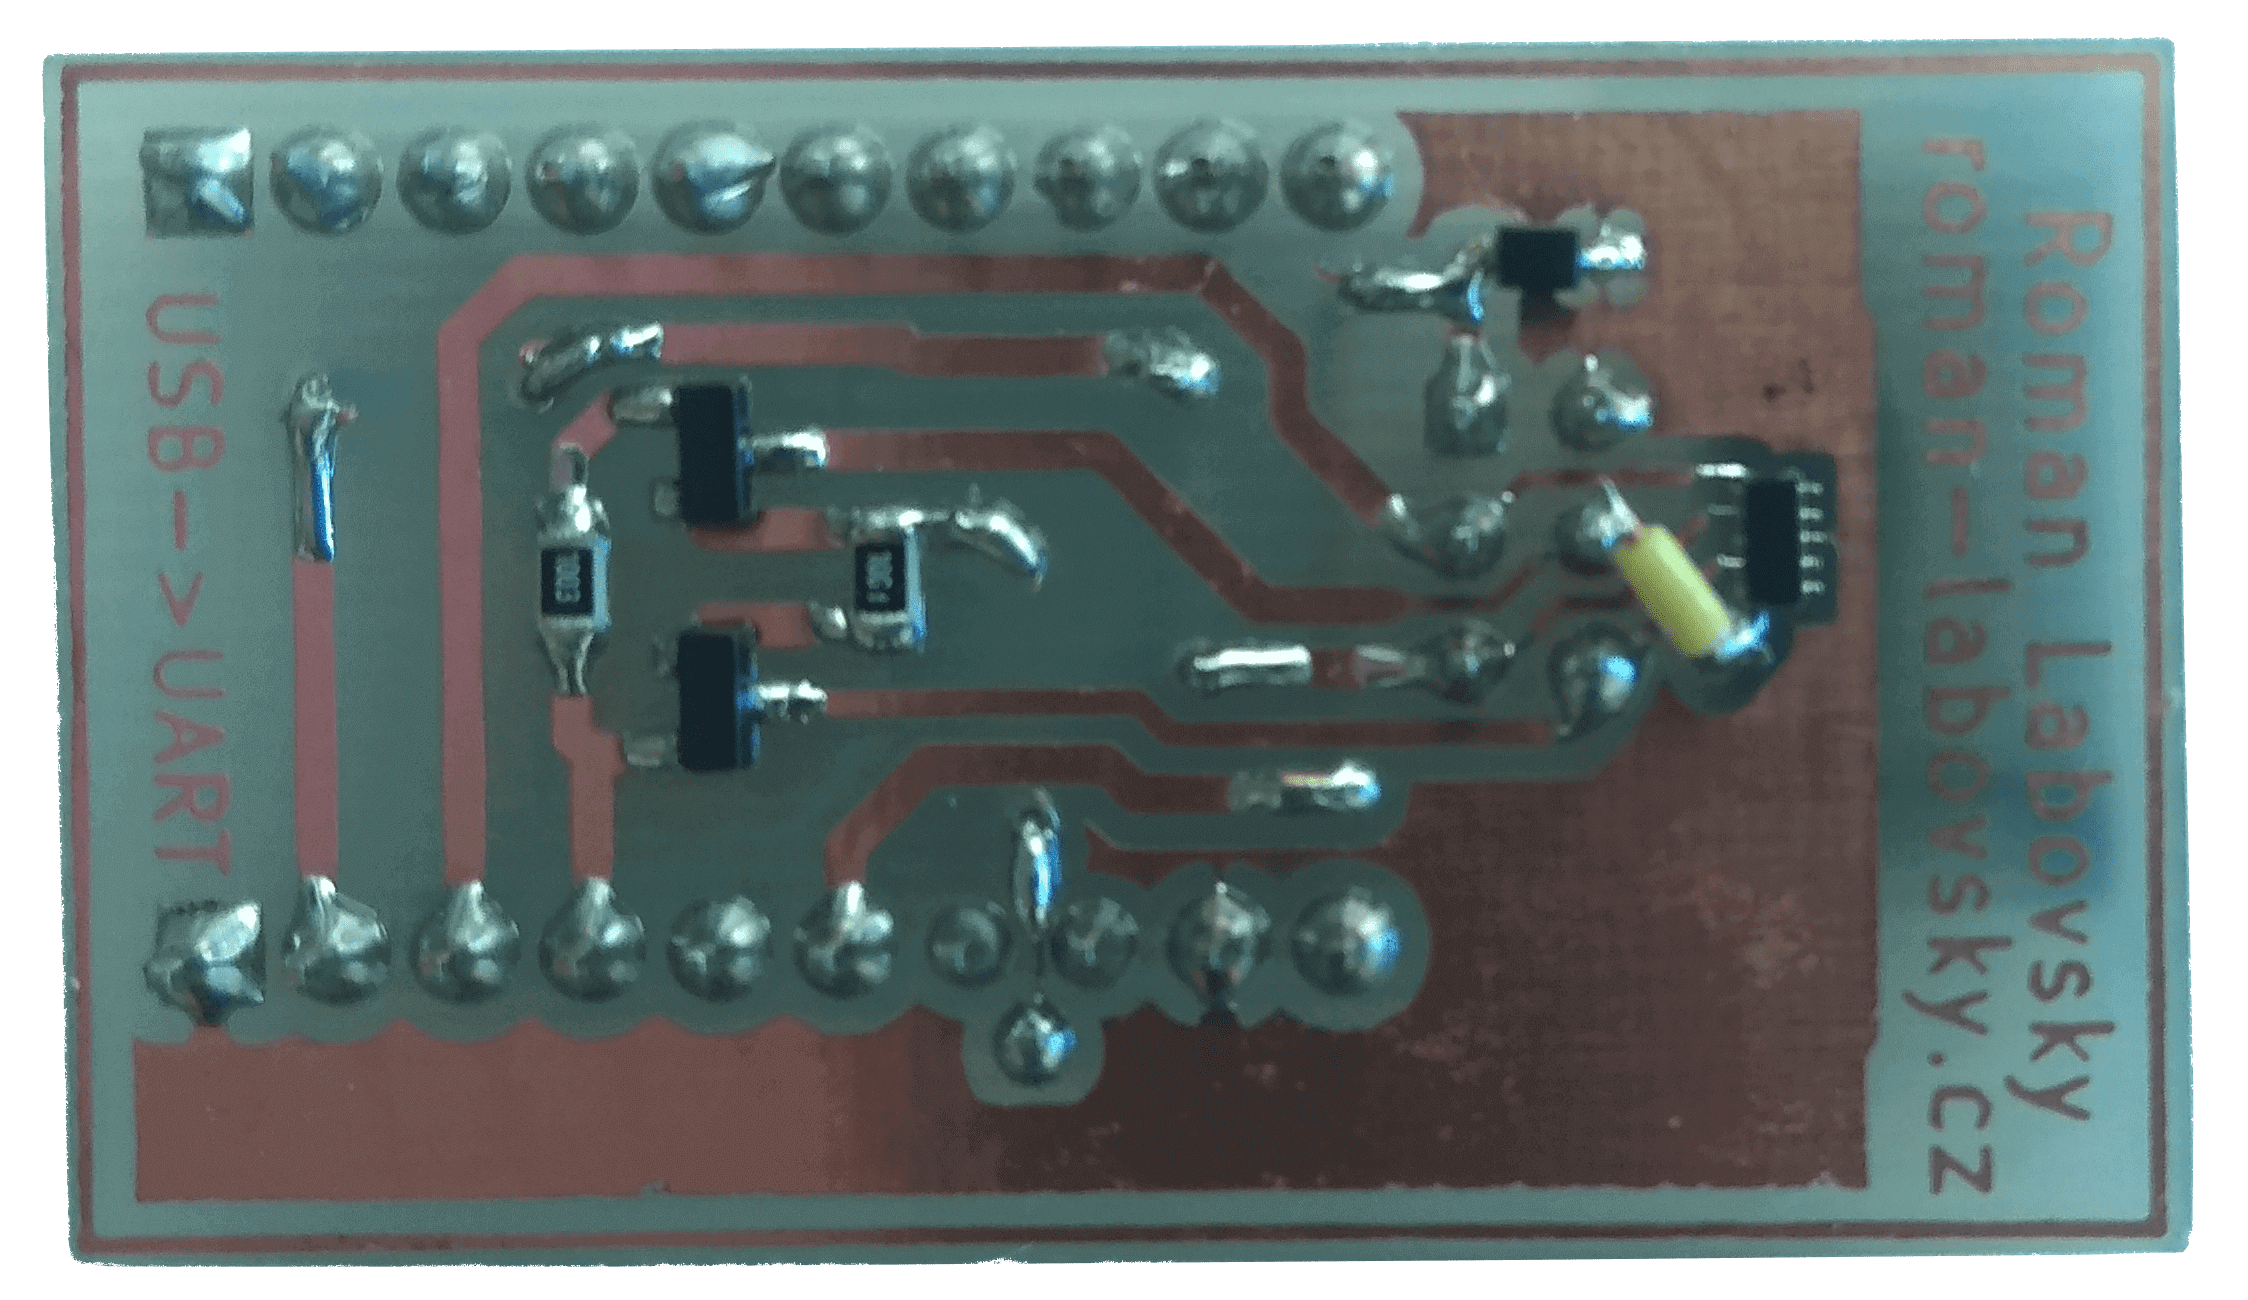
\includegraphics[width=\textwidth]{images/prevodnik-usb-uart-cp2102n/prevodnik-cp2102n-modul-spodni-cast.png}
    \caption[Spodní část modulu převodníku USB-UART.]{Spodní část modulu převodníku USB-UART s~doplněnými tranzistory pro signály DTR a RTS pro automatický bootloader.}
    \label{fig:prevodnik-cp2102n-modul-spodni-cast}
\end{subfigure}
\caption{Převodníku USB-UART CP2102N MINEK.}
\label{fig:prevodnik-cp2102n}
\end{figure}